\documentclass{article}
\usepackage{graphicx} % Required for inserting images
\usepackage{amsmath}

\usepackage{tikz}

\usetikzlibrary{arrows.meta, positioning}
\usepackage{natbib}
\title{Forecasting as Inductive World Modeling}
\author{ }
\date{}
\begin{document}
\maketitle


\newpage

\section{Introduction}
Judgmental forecasting is a demanding form of reasoning about the world. Forecasts about elections, product launches, policy decisions, or geopolitical events require forecasters to move from incomplete and noisy evidence to calibrated beliefs about uncertain future outcomes. Successful forecasters identify relevant base rates, update on new information, reason about interacting actors and institutions, and decompose complex questions into tractable subproblems~\citep{tetlock2016superforecasting,mellers2014psychological}. In this sense, judgmental forecasting provides a natural setting for studying inductive world modeling: the process of generalizing from sparse, noisy observations to infer latent states, mechanisms, and dynamics, and then using those inferred models to predict how the world may evolve~\citep{tenenbaum2006theory,griffiths2010probabilistic}.

Language agents are emerging as strong judgmental forecasters, approaching human forecasting aggregates and rivaling human crowds~\citep{halawi2024approaching, schoenegger2024wisdom}. This success is striking in light of a broader debate over whether sequence prediction induces usable world models~\citep{mitchell2023ai,andreas2024languagemodelsworldmodels}. In a canonical example, OthelloGPT learns to predict legal moves from game transcripts alone, and probing experiments suggest that it internally represents aspects of the board state~\citep{li2023emergent}. Yet recent work by \citet{vafa2025foundation}  complicates this interpretation: foundation models can excel at prediction tasks while failing to develop inductive biases aligned with the underlying world model, including models trained on orbital trajectories that fail to apply Newtonian mechanics to new physics tasks.

This creates a puzzle. On the one hand, accurate forecasts may reflect agents' ability to construct local world models and reason inductively from evidence, echoing expert forecasting practices such as decomposition, base-rate use, and belief updating~\citep{mellers2014psychological,tetlock2016superforecasting}.
On the other hand, accurate forecasts may arise from different strategies, including broad analogical induction over patterns encoded during training, retrieval of similar cases~\citep{kojima2022large,yasunaga2024large}, or other shortcut strategies that succeed on the observed prediction task without recovering an explicit, event-specific world model~\citep{vafa2025foundation}.

This paper uses forecasting as a diagnostic setting for separating these possibilities. We investigate whether language models and language agents construct coherent, updateable event forecasting models. We test this question in three complementary settings. First, we evaluate frontier agents prospectively on unresolved prediction-market questions and test whether their stated hypotheses and forecasts update consistently under targeted evidence interventions. Second, we introduce simulated sequential forecasting worlds where the latent data-generating process is known, allowing us to measure whether models infer hidden states and mechanisms. Third, we test whether forecasting training transfers across synthetic worlds and real forecasting tasks, distinguishing task-specific pattern learning from more general inductive world modeling.

\newpage
\section{Experiment 1: Prospective Forecasting and World-Model Consistency}

\begin{itemize}
    \item We sample newly created or recently active binary Polymarket markets and ask frontier language agents to forecast the probability that each market resolves to \textbf{yes}.
        \begin{itemize}
        \item subset to events that close 14 - 180 days from now
        \item subset to markets that contain a minimum volume of 1000 transactions
        \item subset to events that are `Politics`, `Government`, `Elections`, `Economics`, `Geopolitics`.
        \item subset to markets that are open.
        \item get daily price at CLOB
        \end{itemize}

    \item Markets are unresolved at the time of prediction, reducing the risk that performance reflects memorization of resolved outcomes.
        \begin{itemize}
            \item Subset to 100 questions that are diverse (from the set above)
        \end{itemize}

    \item  For each market, the agent receives the question and resolution criteria, then proposes a structured event model: key actors, institutions, mechanisms, latent variables, and competing hypotheses.
        \begin{itemize}
            \item Agent with Microsoft Azure Foundry -- Chatgpt-5.4 (latest model that I can deploy for basically free)
            \item Agent has web access
            \item 5 independent runs per market (take the median).
        \end{itemize}

    \item  The agent gathers or receives time-available evidence, evaluates how the evidence bears on each hypothesis, assigns subjective probabilities to hypotheses, and maps them to a final forecast.

    \item We construct counterfactual evidence packets that alter the evidence in directionally interpretable ways, such as strengthening support for a candidate, weakening turnout evidence, or changing support from pivotal legislators.

    \item  The agent receives the modified evidence and updates both its hypothesis probabilities and final forecast. This is done by manually modifying the agent's received output.

    \item  We evaluate whether updates are consistent with the agent's stated model:
    \begin{itemize}
        \item \emph{Evidence--hypothesis consistency}: targeted evidence changes the corresponding hypothesis probability in the expected direction.
        \item \emph{Hypothesis--forecast consistency}: changes in hypothesis probabilities imply corresponding changes in the final forecast.
    \end{itemize}

    \item The experiment tests whether accurate forecasts are supported by coherent, updateable event models, or instead arise from shortcuts, post-hoc rationalization, or market imitation.
\end{itemize}

\newpage


\newpage
\begin{figure}[t]
\centering
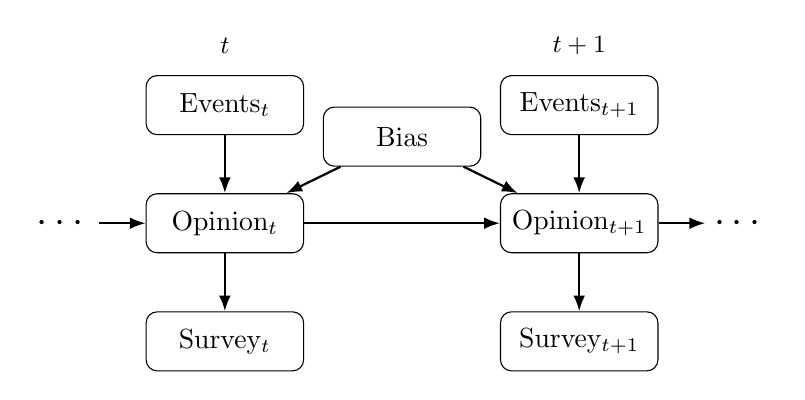
\begin{tikzpicture}[
    node distance=1.25cm and 1.75cm,
    var/.style={
        rectangle,
        rounded corners,
        draw,
        align=center,
        minimum width=2.0cm,
        minimum height=0.75cm
    },
    arrow/.style={-{Latex[length=2mm]}, thick}
]

% Time t
\node[var] (events1) at (0,0.9) {Events$_t$};
\node[var] (opinion1) at (0,-0.6) {Opinion$_t$};
\node[var] (survey1) at (0,-2.1) {Survey$_t$};

% Time t+1
\node[var] (events2) at (4.5,0.9) {Events$_{t+1}$};
\node[var] (opinion2) at (4.5,-0.6) {Opinion$_{t+1}$};
\node[var] (survey2) at (4.5,-2.1) {Survey$_{t+1}$};

% Shared bias node
\node[var] (bias) at (2.25,0.5) {Bias};

% Continuity dots
\node at (-2.05,-0.6) {\Large $\cdots$};
\node at (6.55,-0.6) {\Large $\cdots$};

% Within-time arrows
\draw[arrow] (events1) -- (opinion1);
\draw[arrow] (events2) -- (opinion2);

\draw[arrow] (opinion1) -- (survey1);
\draw[arrow] (opinion2) -- (survey2);

% Temporal persistence
\draw[arrow] (-1.6,-0.6) -- (opinion1);
\draw[arrow] (opinion1) -- (opinion2);
\draw[arrow] (opinion2) -- (6.1,-0.6);

% Bias arrows
\draw[arrow] (bias) -- (opinion1);
\draw[arrow] (bias) -- (opinion2);

% Time labels
\node[font=\small] at (0,1.65) {$t$};
\node[font=\small] at (4.5,1.65) {$t+1$};

\end{tikzpicture}
\caption{Temporal structure of the Biased Election World. Events and bias affect latent opinion at each time step. Opinion persists over time and generates noisy survey results.}
\label{fig:biased-election-temporal-dag}
\end{figure}

\section{Experiment 2: Simulated sequential forecasting tasks}


\subsection{Election World}
\begin{itemize}
    \item  We construct a simulated election environment in which language models forecast the next survey result after observing a sequence of prior events and survey results.

    \item Negative events reduce public opinion, which in turn determines survey results. However, the effect of negative events is moderated by news bias: in cities with biased news coverage, negative events have only a minor effect on public opinion, whereas in cities with neutral coverage, the same events produce larger shifts.

    \item Models do not directly observe news bias or public opinion at any time step. They observe only events and survey results. The latent bias variable is never explicitly revealed.

    \item  In a new sequential forecasting task, the model predicts $\text{Survey}_{t+1}$ from the observed history. Rather than simply averaging past event--survey relationships, a most successful model should form a hypothesis around the latent variable and then maintain uncertainty about whether the city has biased or neutral news coverage and weight its forecast accordingly.

    \item Variations: The pooling company is mentioned,  there is one biased pooling company. We explicitly say the pooling company is owned by the cousing of one of the candidates. We say nothing.  We can also consider other different "synthetic worlds"



\end{itemize}

\newpage


\section{Experiment 3: Training and Transfer Across Synthetic and Real Forecasting Worlds}

\begin{itemize}
    \item We test whether forecasting training improves general inductive world-modeling ability, rather than only performance on the training distribution.

    \item  We evaluate transfer in both synthetic and real-world settings:
    \begin{itemize}
        \item \emph{Synthetic forecasting worlds}: language models forecast future observations in simulated sequential environments where the latent structure is known. We train models on a family of simulated sequential forecasting tasks, leaving one such environment out. We measure performance in the held out environment as training proceeds.

        \item \emph{Real-world pastcasting}: language agents forecast historical Polymarket questions using evidence that would have been available at the time.
        We train models on a family of questions and measure performance on a held out set of quesitons.
    \end{itemize}


\end{itemize}


\bibliographystyle{plainnat}
\bibliography{main}

\end{document}
